\documentclass[a4paper,twoside]{article}
\usepackage[T1]{fontenc}
\usepackage{graphicx}
\usepackage{graphics}
\usepackage{float}
\usepackage[cm]{fullpage}
\pagestyle{myheadings}
\usepackage{etoolbox}
\usepackage{setspace} 
\usepackage{lipsum} 
\usepackage[bahasa]{babel}
\setlength{\headsep}{30pt}
\usepackage[inner=2cm,outer=2.5cm,top=2.5cm,bottom=2cm]{geometry} %margin
% \pagestyle{empty}

\makeatletter
\renewcommand{\@maketitle} {\begin{center} {\LARGE \textbf{ \textsc{\@title}} \par} \bigskip {\large \textbf{\textsc{\@author}} }\end{center} }
\renewcommand{\thispagestyle}[1]{}
\markright{\textbf{\textsc{AIF401/AIF402 \textemdash Rencana Kerja Skripsi \textemdash Sem. Genap 2016/2017}}}

\newcommand{\HRule}{\rule{\linewidth}{0.4mm}}
\renewcommand{\baselinestretch}{1}
\setlength{\parindent}{0 pt}
\setlength{\parskip}{6 pt}

\onehalfspacing
 
\begin{document}

\title{\@judultopik}
\author{\nama \textendash \@npm} 

%tulis nama dan NPM anda di sini:
\newcommand{\nama}{Evelyn Wijaya}
\newcommand{\@npm}{2015730030}
\newcommand{\@judultopik}{Open Source Snake 360} % Judul/topik anda
\newcommand{\jumpemb}{1} % Jumlah pembimbing, 1 atau 2
\newcommand{\tanggal}{05/09/2018}

% Dokumen hasil template ini harus dicetak bolak-balik !!!!

\maketitle

\pagenumbering{arabic}

\section{Deskripsi}
Snake merupakan sebuah permainan yang pertama kali dibuat oleh Peter Trefonas pada tahun 1978. Konsep Snake pertama kali berasal dari permainan arkade yaitu Blockade. Pada saat itu, Snake hanya dapat dimainkan pada komputer pribadi saja. Pada tahun 1997, Snake dapat dimainkan pada telepon genggam Nokia \footnote{https://en.wikipedia.org/wiki/Snake\_(video\_ game\_ genre)}.\\\\
Cara bermainya cukup mudah yaitu pemain mengendalikan ular untuk mendapatkan makanan tanpa menabrak rintangan atau ular itu sendiri. Setiap memakan makanan, kita akan mendapat skor dan tubuh ular akan memanjang. Apabila ular tersebut menabrak dirinya sendiri atau menabrak rintangan, maka permainan selesai.\\\\
Sekarang, sudah banyak sekali permainan Snake yang dapat dimainkan di smartphone dan web browser. Bahkan pergerakan ular juga tidak hanya 4 arah saja(atas, bawah, kiri dan kanan), tetapi sudah dapat bergerak ke segala arah. Selain itu, permainan Snake ini juga dapat dimainkan lebih dari 1 orang, contohnya adalah Slither.io. \\\\
Pada skripsi ini akan dibuat permainan Snake yang ularnya dapat bergerak ke segala arah dan orang lain dapat menambahkan pilihan labirin. Permainan Snake akan dibuat menggunakan HTML5/Canvas dan menambah pilihan labirin menggunakan mekanisme pull request pada Gitlab.

\begin{figure}[H]
\caption{Pergerakan ular ke segala arah}
\centering
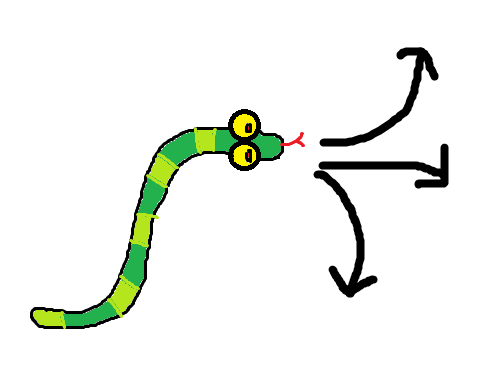
\includegraphics[width=0.5\textwidth]{snake.png}
\end{figure}

\section{Rumusan Masalah}
\begin{itemize}
	\item Bagaimana cara membangun permainan Snake menggunakan HTML5? 
	\item Bagaimana cara agar ular dapat bergerak ke segala arah?
	\item Bagaimana cara menggambar tubuh ular menggunakan HTML5?
	\item Bagaimana cara menyimpan labirin pada file eksternal?
	\item Bagaimana cara menambah labirin menggunakan pull request pada Gitlab?
\end{itemize}

\section{Tujuan}
\begin{itemize}
	\item Dapat membangun permainan Snake menggunakan HTML5. 
	\item Dapat menggerakan ular ke segala arah.
	\item Dapat menggambar tubuh ular menggunakan HTML5.
	\item Dapat menyimpan labirin pada file eksternal.
	\item Dapat menambah labirin menggunakan pull request pada Gitlab.
\end{itemize}

\section{Deskripsi Perangkat Lunak}
Perangkat lunak akhir yang akan dibuat memiliki fitur minimal sebagai berikut:
\begin{itemize}
	\item Pengguna dapat menggerakan ular ke segala arah dalam permainan Snake tersebut. 
	\item Pengguna dapat menambahkan labirin menggunakan mekanisme pull request pada Gitlab yang dapat disimpan pada file eksternal.
\end{itemize}

\section{Detail Pengerjaan Skripsi}
Bagian-bagian pekerjaan skripsi ini adalah sebagai berikut :
	\begin{enumerate}
		\item Melakukan studi literatur mengenai HTML5, Javascript dan JQuery.
		\item Melakukan analisis dan menentukan objek-objek pada permainan Snake.
		\item Merancang alogritma untuk menggambar tubuh ular, pergerakan ular dan membuat labirin.
		\item Mengimplentasikan keseluruhan algoritma.
		\item Menambahkan labirin menggunakan pull request pada Gitlab.
		\item Melakukan pengujian dan debugging.
		\item Menulis dokumen skripsi.
	\end{enumerate}

\section{Rencana Kerja}
Rincian capaian yang direncanakan di Skripsi 1 adalah sebagai berikut:
\begin{enumerate}
\item Melakukan studi literatur mengenai HTML5, Javascript, dan JQuery.
\item Melakukan analisis dan menentukan objek-objek pada permainan Snake.
\item Merancang algoritma untuk menggambar tubuh ular dan pergerakan ular.
\item Mengimplementasikan algoritma untuk menggambar tubuh ular dan pergerakan ular.
\end{enumerate}

Sedangkan yang akan diselesaikan di Skripsi 2 adalah sebagai berikut:
\begin{enumerate}
\item Merancang algoritma untuk membuat labirin. 
\item Mengimplementasikan algoritma untuk membuat labirin.
\item Menambahkan labirin menggunakan pull request pada Gitlab.
\item Melakukan pengujian dan debugging.
\item Menulis dokumen skripsi.
\end{enumerate}

\vspace{1cm}
\centering Bandung, \tanggal\\
\vspace{2cm} \nama \\ 
\vspace{1cm}

Menyetujui, \\
\ifdefstring{\jumpemb}{2}{
\vspace{1.5cm}
\begin{centering} Menyetujui,\\ \end{centering} \vspace{0.75cm}
\begin{minipage}[b]{0.45\linewidth}
% \centering Bandung, \makebox[0.5cm]{\hrulefill}/\makebox[0.5cm]{\hrulefill}/2013 \\
\vspace{2cm} Nama: \makebox[3cm]{\hrulefill}\\ Pembimbing Utama
\end{minipage} \hspace{0.5cm}
\begin{minipage}[b]{0.45\linewidth}
% \centering Bandung, \makebox[0.5cm]{\hrulefill}/\makebox[0.5cm]{\hrulefill}/2013\\
\vspace{2cm} Nama: \makebox[3cm]{\hrulefill}\\ Pembimbing Pendamping
\end{minipage}
\vspace{0.5cm}
}{
% \centering Bandung, \makebox[0.5cm]{\hrulefill}/\makebox[0.5cm]{\hrulefill}/2013\\
\vspace{2cm} Nama: \makebox[3cm]{\hrulefill}\\ Pembimbing Tunggal
}
\end{document}

